\chapter{Test and Evaluation}
\label{ch:evaluation}
%Aufbau der Messumgebung, see docker-deploy
%Server/Betriebssystem etc.,Datensätze,
%Anfragen, Systeme/Ansätze gegen die Sie sich vergleichen,
%Wie messen Sie? Methodik und Maßeinheiten?
\section{Local test environment}

Unit- and Integration tests, IT needs docker infrastructure, usually mocked JMX, REST data,
lack of time, test separation via naming *Test and *IT via Maven Failsafe, check test coverage,

\section{Docker environment}

Short Docker intro, benefits in microservice environments, describe setup for components (docker-compose.yml),
describe modifications made for Apache Flink and Apache Kafka to enable JMX remote access

\begin{figure}[H]
	\centering
	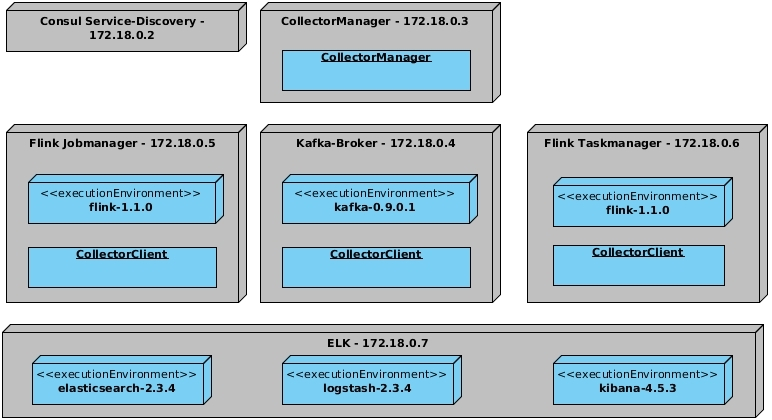
\includegraphics[width=1.0\textwidth]{../uml/deployment-diagram.jpg}
	\caption{Docker Deployment diagram}
	\label{img:deployment-diagram}
\end{figure}

\section{Observations}

CollectorDataProcessor: module to analyze the data streams creating derived streams and persist flat
data -> data transformation, analytics layer

Kibana dashboard, show visualization of CollectorDataProcessor data

\section{Discussion}
%Wurden Sie überrascht? Stimmten Ihre Hypothesen? Sind Sie besser, anders als das andere System?
%Wichtigster Erkenntnisgewinn 1
%Wichtigster Erkenntnisgewinn 2
%Wichtigster Erkenntnisgewinn N
%Anwendbarkeit? Szenario?
\section{Summary}

TODO

%Beschreibung  der Ergebnisse, Diagramme, Darstellen von Zusammenhängen